\chapter{Introduction}
\minitoc\vspace{.5cm}

\section{Motivation}
% Start describing the situation as it is today or as it has been during the last years. ’Over
% the last few years there has been a tendency... In recent years...’. The introduction
% should make people aware of the problem that you are trying to solve with your concept,
% respectively implementation. Don’t start with ’In my thesis I will implement X’.

% Research Context - Forschungskontext
% -- IoT
The \ac{IoT} is one of the biggest topics in the recent years.
Companies with a focus in that area have an enormous market growth with plenty of new opportunities, use cases, technologies, services and devices.
Bain \& Company predicts an annual revenue of \$450 billion for companies who selling hardware, software and comprehensive solutions in the \ac{IoT} context by 2020.\autocite{Bosche:2016}
In order to limit the vast area of \ac{IoT}, more and more standards are defined and subtopics established.
The \ac{IERC} divided them into eight categories: Smart Cities, Smart Health-care, Smart Transport and Smart Industry, also known as Industry 4.0, to mention only a few.\autocite[cf.][p. 7]{IERC:2011}
All of them are well connected, for example a Smart Factory, which is a part of the Smart Industry, can get a delivery from a self driving truck (Smart Transport) which navigates through a Smart City to get to the factory.
Such information networks are one of the main goals of \ac{IoT}.
% Research Area - Forschungsgebiet
% -- Smart Factories
In the Industry 4.0 for example, multiple smart factories should be interconnect into a distributed and autonomous value chain.
Also, the automation level in a single factory will be increased which helps to have a more flexible and efficient production process.
Currently a factory has a high degree of automation, but due to a lack of intelligence and communication between the machines and the underlying system, they can not react to changing requirements or unexpected situations.
% Application Area - Anwendungsbereich
% -- CS & CPS
One solution to achieve that are \acp{CPS}.
These are virtual systems which are connected with embedded systems to monitor and control physical processes.\autocite[cf.][p. 363]{Lee:2008}
A normal \ac{CS} is passive, means it could not interact with the physical world, with the appearance of \acp{CPS} things can communicate so the system has significantly more intelligence in sensors and actuators.\autocite[cf.][p. 1363 f.]{Poovendran:2010}
% Research Focus - Forschungsschwerpunkt aka Praxisproblem
% -- Virtualization, Orchestration, Deployment of functions
\newpage
Another solution is to change the fundamental architecture of such a system from a monolithic to more distributed architecture.
With Fog Computing the cloud moves away from centralized data centers to the edge of the underlying network.\autocite[cf.][p. 380]{Pahl:2015}
Such a network can have thousands of nodes with multiple sensors, machines or smart components connected to them.
An "intermediate layer between the IoT environment and the Cloud"\autocite[p.236]{Brito:2016} enables a lot of new possibilities like pre-computation and storage of gathered data.
This reduces traffic and the resource overhead in the cloud, it keeps sensitive data on-premise\autocite[cf.][p.236]{Brito:2016} and enables real-time applications to take decisions based on analytics running near the device.
It also can achieve lower the network latency.
On the other hand there are also a lot of challenges in these highly heterogeneous and hybrid environment.
As an example in some scenarios multiple low power devices have to interact with each other, lossy signals and short range radio technologies are widely used and nodes can appear and disappear frequently.\autocite[cf.][p. 325]{Yannuzzi:2014}
Especially the last case is elaborated because the underlying system has to handle that.
Furthermore the required applications running on these nodes can be changed often and have to be deployed and removed in a dynamical way.

\acp{VM} are a common approach in Cloud systems to provide elasticity of large-scale shared resources.\autocite[cf.][p. 117]{Pahl:2016}
A more lightweight, less resource and time consuming solution is container virtualization.
"Furthermore, they are flexible tools for packaging, delivering and orchestration software infrastructure services as well as application"\autocite[p. 117]{Pahl:2016}.
Orchestration tools like Kubernetes\footnote{\url{https://kubernetes.io}} and Docker Swarm\footnote{\url{https://docs.docker.com/engine/swarm}} that can deploy, scale and manage containers to clusters of hosts have become established in the last years.
If this technology can be applied to the \ac{IoT} area, many challenges can be solved.
Dynamically deployed applications at the edge of a network can store and preprocess gathered data even if a node have no connection to the cloud.
Traffic can be reduced by only transmitting aggregated data back to the cloud.
Lossy signals can be compensated due to an autonomous behavior of the different components.
More often small low power devices with a limited computational power are used as \ac{IoT} devices which also profit rather from lightweight container solutions than from resource consuming \acp{VM}.
This thesis shows the possibilities of container orchestration for the \ac{IoT} and smart factories by creating a prototypical implementation of an orchestration engine that can be executed on fog nodes.
Therefore an engine will be created that can orchestrate containers based on functional and non-functional constraints onto a single fog node or between a cluster of fog nodes.


\section{Objective}
% What kind of problem do you adress? Which issues do you try to solve? What solution
% do you propose? What is your goal? ’This thesis describes an approach to combining X
% and Y... The aim of this work is to...’

% write about the first issue
% -- deployment of applications

% write about the second issue
% -- detect constraints

% write about the synopsis (Zusammenfassung) of the issues
This thesis describes an approach to design and implement a fog service orchestration engine for smart factories.
The aim of this work is to create a prototypical implementation of an orchestration engine for a fog node, hereinafter called prototype, that can deploy containers on the same node or on other network nodes.
A fog Node can be a low power device at the edge of a network, especially in the area of Industry 4.0 and smart factories.
Furthermore the prototype should consider specific functional and non-functional constraints while deploying the containers.
A condition can be a hardware requirement, a required software or a dependencies to another node.
The technical prerequisite and detailed requirements for the prototype as well as the usability of a \ac{GUI}, which could be for example Open Baton, an \ac{ETSI} \ac{NFV} compliant \ac{MANO} framework, have to be worked out.
The cooperation with the \ac{FOKUS} plays a prominent role for this thesis, because of their knowledge and experience in the area of \ac{IoT} and \ac{NFV}.
As the development method of choice a Kanban like process will be used.
Kanban is flexible but also straight forward.
There is less meeting overhead then in Scrum, but it also helps to have an eye on the planed and spend resources.


\section{Scope}
% Here you should describe what you will do and also what you will not do. Explain a
% little more specific than in the objective section. ’I will implement X on the platforms
% Y and Z based on technology A and B.’
% Conclude this subsection with an image describing ’the big picture’. How does your
% solution fit into a larger environment? You may also add another image with the overall
% structure of your component.
% ’Figure 1.1 shows Component X as part of ...’

% write about the research assumptions (Forschungsannahmen)
% -- haypothese, was ist der erwartete outcome?

% write about the research scope (Forschungsbereich) — Figures 1.1, 1.2 and 1.4
% -- was ist drin, was nicht
As mentioned before, the engine to be developed will be a prototype for a fog node.
Open Baton serves as the template for that project and especially the modular architecture and the resulting extensibility will be targeted.
Beside that, the whole prototype will be created completely from scratch.
The container virtualization will be realized with Docker\footnote{\url{https://www.docker.com}}, an open source container platform.
Docker has on \ac{API} where third party apps can communicate with and can control the engine himself.
The functional and non-functional constraints can be stored and transfered for example as \ac{YAML} schemes which are part of the \ac{TOSCA} standard.
These schemes should be extendable and should fit the needs of the constraint functionality.

\begin{figure}[H]
    \centering
    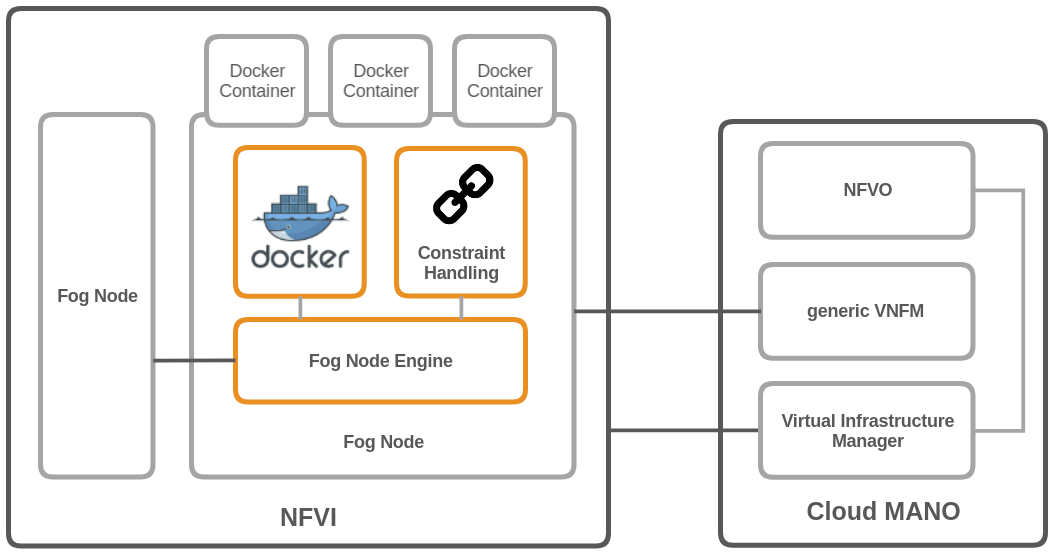
\includegraphics[width=0.85\textwidth]{resources/images/conceptual_architecture.png}
    \caption[Conceptual architecture based on a draft of the \ac{FOKUS}]{Conceptual architecture based on a draft of the FOKUS}
    \label{fig:conceptual_architecture}
\end{figure}

Figure \ref{fig:conceptual_architecture} shows a conceptual architecture design that based on a draft of the \ac{FOKUS}.
On the right side is the abstract cloud infrastructure.
These could be for example Open Baton or any other \ac{MANO} compliant Framework.
The cloud infrastructure will be considered while developing the prototype, but the development or integration of such a component is out of scope for this thesis.
The \ac{NFVI} on the left side includes the Fog Node.
A single fog node should have the fog node engine, which is the prototype to be developed, as well as the Docker engine.
The constraint handling is part of the fog node engine and the concrete implementation has to be elaborated.
The fog node engine can orchestrate the local Docker containers, or if it necessary, it can move containers over to one or multiple other fog nodes.
This allows the system to be more flexible and it can achieve an autonomous orchestration level.
The autonomous orchestration of containers between fog nodes without an existing connection to the cloud server is desirable, but not part of this thesis.
Due to the fact that the prototype will be used in an \ac{IoT} context, the system will be tested on low power devices, for example on a Raspberry Pi\footnote{\url{https://www.raspberrypi.org}} cluster.
It is out of scope to create a system that guarantee to be executable on arbitrary devices, but theoretically this could be achieved by using platform an independent programming language and corresponding frameworks.


\section{Outline}
In chapter \ref{chapter:state-of-the-art} an introduction into relevant topics like the \ac{IoT} in the context of Industry 4.0, \acp{CPS} and Fog Computing as subtopics, virtualization, especially container virtualization and orchestration and \ac{NFV} is given.
Followed by a comparison of several established tools available on the market and finally some messaging concepts like \ac{MQTT} and ZeroMQ.
The definition of the requirements as well as features and capabilities of the prototype will be shown in chapter \ref{chapter:requirements-analysis}.
Based on that, the architecture of the system is illustrated in chapter \ref{chapter:concept}.
The proof-of-concept implementation will be worked out in chapter \ref{chapter:implementation} and the functionality of the plugin will be demonstrated.
Chapter \ref{chapter:evaluation} summarizes the results of the work and evaluates the viability in terms of software quality, usability and feature-completeness.
Finally the gathered insights as well as an outlook for further improvements of the plugin will be argued in chapter \ref{chapter:conclusion}.
% TODO: can be more detailed

% The ’structure’ or ’outline’ section gives a brief introduction into the main chapters of
% your work. Write 2-5 lines about each chapter. Usually diploma thesis are separated
% into 6-8 main chapters.
% This example thesis is separated into 7 chapters.
% Chapter 2 is usually termed ’Related Work’, ’State of the Art’ or ’Fundamentals’.
% Here you will describe relevant technologies and standards related to your topic. What
% did other scientists propose regarding your topic? This chapter makes about 20-30 percent
% of the complete thesis.
% Chapter 3 analyzes the requirements for your component. This chapter will have
% 5-10 pages.
% Chapter 4 is usually termed ’Concept’, ’Design’ or ’Model’. Here you describe your
% approach, give a high-level description to the architectural structure and to the single
% components that your solution consists of. Use structured images and UML diagrams
% for explanation. This chapter will have a volume of 20-30 percent of your thesis.
% Chapter 5 describes the implementation part of your work. Don’t explain every code
% detail but emphasize important aspects of your implementation. This chapter will have
% a volume of 15-20 percent of your thesis.
% Chapter 6 is usually termed ’Evaluation’ or ’Validation’. How did you test it? In
% which environment? How does it scale? Measurements, tests, screenshots. This chapter
% will have a volume of 10-15 percent of your thesis.
% Chapter 7 summarizes the thesis, describes the problems that occurred and gives an
% outlook about future work. Should have about 4-6 pages.

% write about the research outline and Figure 1.6. Summarize Chapters 1 to 8
